\documentclass[10pt]{article}
\usepackage[usenames]{color} %used for font color
\usepackage{amssymb} %maths
\usepackage{amsmath} %maths
\usepackage[utf8]{inputenc} %useful to type directly diacritic characters
\usepackage{tikz}
\usetikzlibrary{arrows,positioning,decorations.pathreplacing} 

\definecolor{boiseBlue} {RGB}{29,72,159}
\definecolor{rojoAmor} {RGB}{171,13,4}
\definecolor{moradoAmor} {RGB}{93,8,113}
\definecolor{verdeAmor} {RGB}{98,158,31}
\definecolor{negro} {RGB}{10,10,10}
\definecolor{lgreen} {RGB}{180,210,100}
\definecolor{dblue}  {RGB}{20,66,129}
\definecolor{ddblue} {RGB}{11,36,69}
\definecolor{lred}   {RGB}{220,0,0}
\definecolor{nred}   {RGB}{224,0,0}
\definecolor{norange}{RGB}{230,120,20}
\definecolor{nyellow}{RGB}{255,221,0}
\definecolor{ngreen} {RGB}{98,158,31}
\definecolor{dgreen} {RGB}{78,138,21}
\definecolor{nblue}  {RGB}{28,130,185}
\definecolor{jblue}  {RGB}{20,50,100}\begin{document}
\[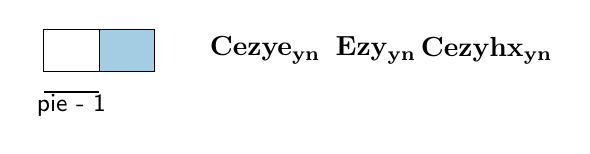
\begin{tikzpicture}
%
\node[draw=black,minimum width=4em,minimum height=1.5em,rectangle]  at (0,0) {};
\node[draw=black,fill=nblue!40,minimum width=2em,minimum height=1.5em,rectangle]  at (1em,0em) {}; % height=4em
%
\node[]  at (6em,0) {${\bf Cezye_{yn}}$};
\node[]  at (10em,0) {${\bf Ezy_{yn}}$};
\node[]  at (14em,0) {${\bf Cezyhx_{yn}}$};
%\node[]  at (14em,0) {$+ \; =$};
%
\draw[] (-2em,-1.5em) -- (0em,-1.5em);
\node[]  at (-1em,-2em) {\small{\sf pie - 1}};
%\draw[] (-2em,1.5em) -- (1em,1.5em);
%\node[]  at (-0.5em,2em) {\small{\sf pie - 2}};
%
\end{tikzpicture}
%\\\\
%\odot \;\; = \;\; \dots \;\; + \;\; - \;\; (\]
\]
\end{document}